\section{Results}\label{sec:results}

\subsection{Overall, No Index, 3 Nodes}\label{subsec:overall,NoIndex,3Nodes}
\begin{figure}
    \centering{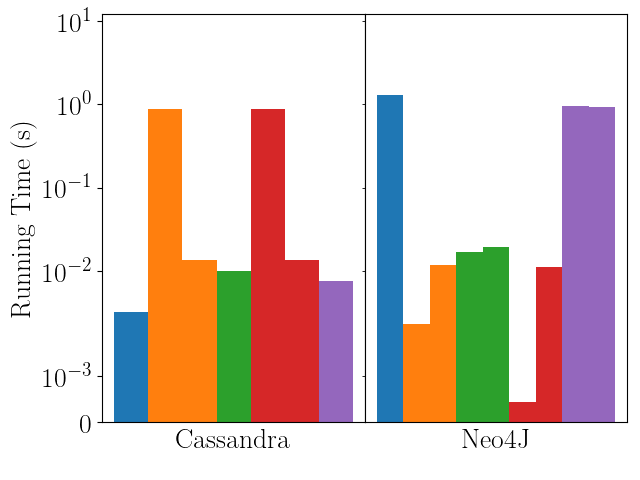
\includegraphics[scale=0.55]{images/qall-3node-none.png}}
    \caption{Running times of different queries for a 3-node Neo4J cluster and a 3-node Cassandra cluster.
    Each point represents the average of 15 runs, executed after 30 runs to warm the cache.
    The blue queries represent query 1, the orange represent queries 2A and 2B, the green represent queries 3
    (Cassandra), 3A, and 3B (Neo4J), the red represents queries 4A and 4B, and the purple represent queries 5
    (Cassandra), 5A, and 5B (Neo4J).}\label{fig:ono3n}
\end{figure}

In~\autoref{fig:ono3n}, all queries are plotted against time for both Neo4J and Cassandra.
Each cluster consists of 3 nodes, a no indexes are applied to any column.

A cursory glance reveals that the time to query a Neo4J cluster is a lot more dispersed than a Cassandra query.
The average deviation of eac
